Based on the \textbf{acf} and \textbf{pacf} in part (a), fit an appropriate ARMA model using \texttt{sarima(p,d,q)} function in R, performing all necessary diagnostics. Comment.

\nl Since the ACF tails off, the model shouldn't be an $\MA(q)$. Since the PACF cuts off after lag $2$, the model could be an $\AR(2)$. This can be fitted with
$$\texttt{sarima(lake,2,0,0, no.constant=TRUE)}.$$
The results of this model are 
\notab{\center{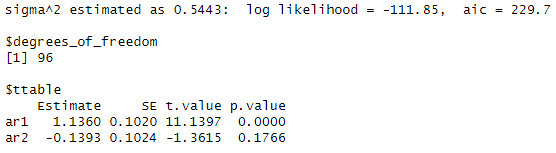
\includegraphics[width=5in]{img/6ar2.PNG}}}
whereby the p-value of one of the coefficients is $0.1766$, which is relatively high, and we want low values. Looking further at the graphs for the model, the ACF of the residuals peaks outside and the Ljung-Box indicates non iid residuals since $\alpha < 0.05$ on some datapoints. The AIC was $229.7$ with $\sigma^2 = 0.5443$, which is fine. 

\notab{\center{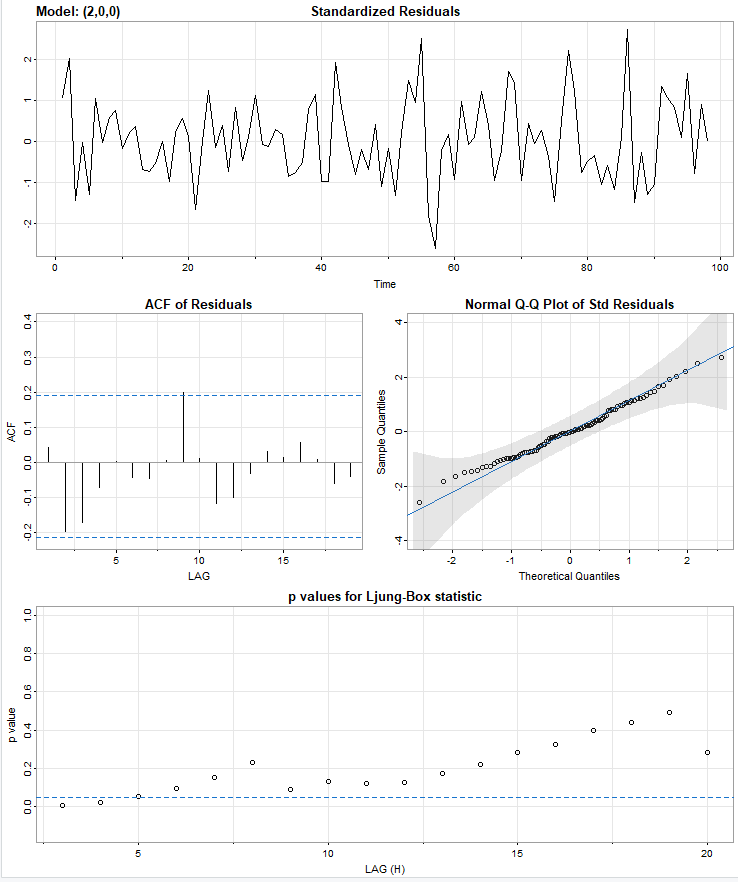
\includegraphics[width=6in]{img/6ar2info.PNG}}}

\nl Moving on to a different model to try and get IID residuals, we can see that the PACF drops even sharper after lag 3, and has almost a large enough drop off after lag 1.

\nl Lag 1 gives good p-values for the coeffient ($p=0$), and has a similar $\sigma^2 = 0.5547$ and AIC of $229.54$. 
\notab{\center{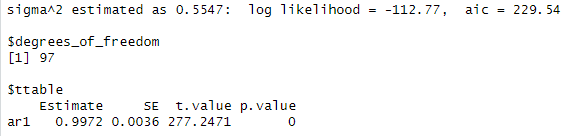
\includegraphics[width=5in]{img/6ar1.PNG}}}

\nl The same problems appear with the diagnostic graphs, though. The Ljung-Box statistic indicates the residuals are not iid and the ACF still spikes. 

\notab{\center{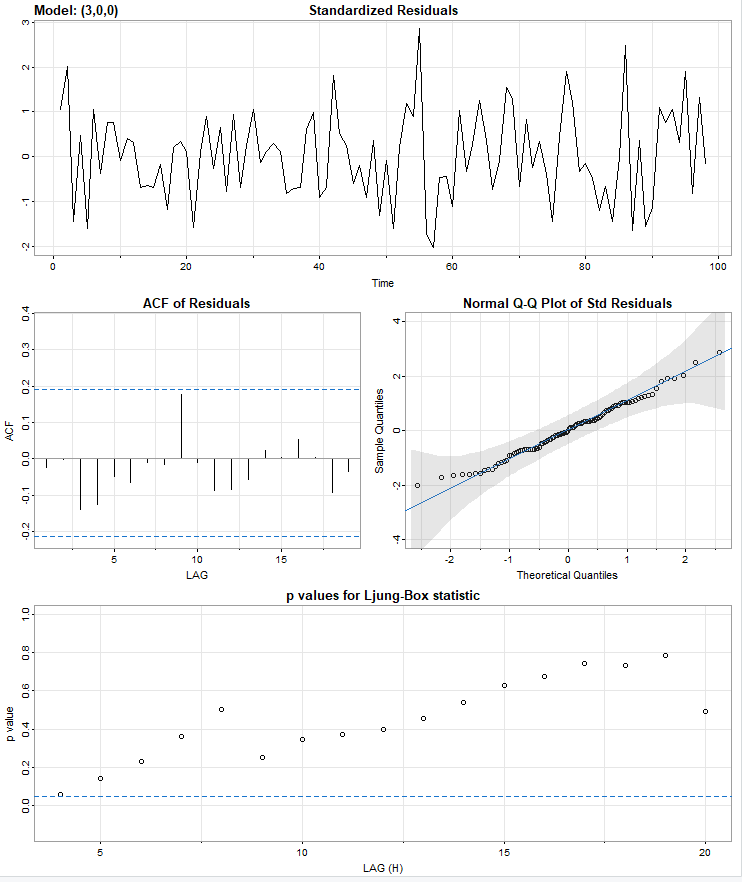
\includegraphics[width=6in]{img/6ar3info.PNG}}}

\nl Finally we settle on Lag 3 because the coefficients are all relatively small with 0.03 being the  max. $\sigma^2 = 0.5183$ is the lowest so far, and same with the AIC of $227.06$. 

\notab{\center{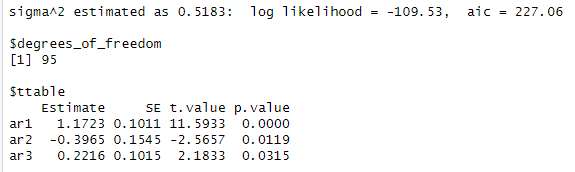
\includegraphics[width=5in]{img/6ar3.PNG}}}

\nl Additionally, the diagnostic graphs are promising too. The Ljung-Box statistic indicates the residuals are iid and the ACF of the residuals has the least spikes of all the tested models. The QQ plot is also a little more normal. For this reason we can conclude that $\AR(3)$ is a good fit for the model. It should be noted that while $\AR(4)$ has a better $\sigma^2$, AIC, and Ljung Box statistic, the p-values of the coefficients are bad, with one of them being 0.80. First differencing also suffered from bad p-values on the coefficients on AR(2) and AR(3), but had lower AICs around 217. Their predictions were flat lines however, so I will ignore those models

\notab{\center{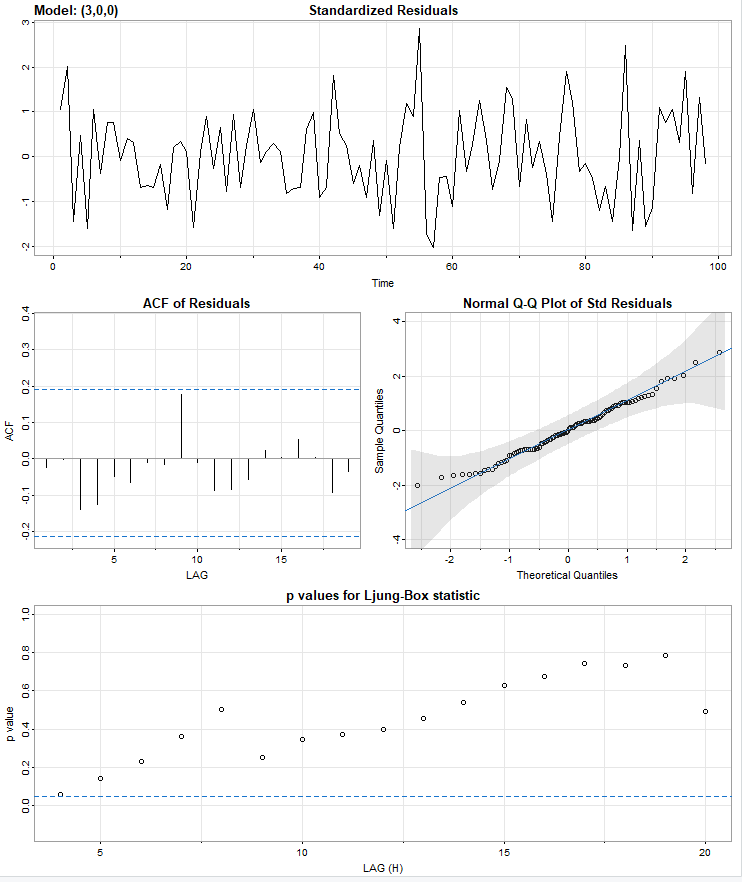
\includegraphics[width=5in]{img/6ar3info.PNG}}}

